\documentclass[12pt]{article}
\usepackage[a4paper, margin=.30in]{geometry}
\usepackage{graphicx ,
            wrapfig,
            xcolor, 
            enumerate,
            amsmath,fontenc,
            tcolorbox
            }
\usepackage{mathptmx}

\newcommand\headerMe[2]{\noindent{}#1\hfill#2}
\renewcommand{\thesection}{\Roman{section}}

\author{Zakaria HAOUZAN}
\date{\today}

\begin{document}
% headers --------------
\headerMe{Matière : Physique-Chimie}{Professeur : Zakaria HAOUZAN}\\
\headerMe{Unité : Electricité}{Établissement : Lycée SKHOR qualifiant}\\
\headerMe{Niveau : 1BAC-SM}{Heure : 5H}\\

% ------Content ________
\begin{center}

    \Large{Leçon $N^{\circ} 7 $: \color{red} Energie potentielle électrostatique (Sc.Math) }
\end{center}

%\begin{wrapfigure}[10]{r}{0.5\textwidth}
    %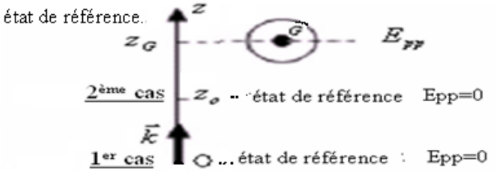
\includegraphics[width=0.5\textwidth]{./img/img00.png}
%\end{wrapfigure}

\begin{wrapfigure}[10]{r}{0.3\textwidth}
  \vspace{-1cm}
    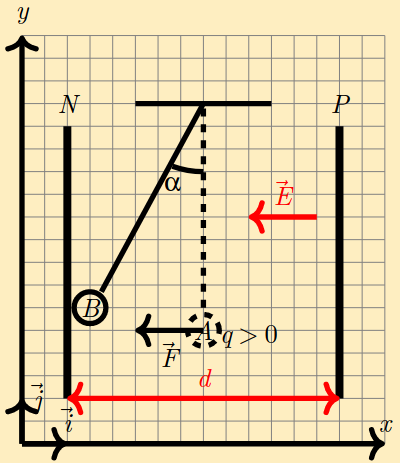
\includegraphics[width=0.3\textwidth]{./img/img_00.png}
\end{wrapfigure}


\section{Travail d’une force électrostatique dans un champ uniforme :}
\subsection{ Activité :}
On place un pendule électrostatique ente deux plaques conductrices planes et parallèles séparées d'une distance d, la boule du
pendule porte une charge $q>0$.

A l’absence du champ électrique la boule se trouve au point M (le pendule est vertical).

 Lorsqu’on applique une tension électrique entre les deux plaques A et B, un champ électrostatique 
 uniforme $\vec{E}$ se crée et la charge q se trouve soumise à une force
électrique $\vec{F} = q.\vec{E}$ ce qui la déplace d’un point A vers un point B .
Puisque le champ est uniforme donc la force $\vec{F}$ est constante.
Dans le repère orthonormé $(O, \vec{i}, \vec{j})$ .
\\--Trouver l’expression du travail de la force $\vec{F}$ lorsque la charge se déplace de M vers N .
On sait que le travail de la force $\vec{F}$ au cours de déplacement de A
vers B est : $$W_{A\rightarrow B}(\vec{F}) = \vec{F}.\vec{MN} = q\vec{E}.\vec{MN}$$
\begin{center}
  \color{blue}
  Dans le repère$ (O, \vec{i},\vec{j})$
  $$\overrightarrow{MN} = (x_M - x_N)\vec{i} + (y_M - y_N)\vec{j}$$
  $\vec{E} = -E\vec{i}$
  $$W_{A\rightarrow B}(\vec{F}) = \vec{F}.\vec{MN} = qE.(x_M - x_N) $$

\end{center}

\section{Potentiel électrique  : }
\subsection{Définition de la différence de potentielle électrique (d.d.p)}
La différence de potentielle ou tension électrique entre deux points
A et B d’une région où règne un champ électrique uniforme $\vec{E}$ , est
égale au produit scalaire des vecteurs $\vec{E}$ et  $\vec{AB}$ :
\fbox{$V_A - V_B = \vec{E}.\overrightarrow{AB}$}
\\Remarque : Cette relation ne s’applique que si le champ
électrique est uniforme.

%\begin{center}
    %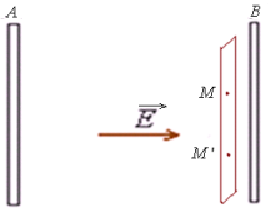
\includegraphics[width=0.5\textwidth]{./img/img_01.png}
%\end{center}

\subsection{ Potentiel électrique: }

  Dans le repère$ (O, \vec{i},\vec{j})$
  $V_A - V_B = \vec{E}.\overrightarrow{AB}.E(x_A - x_B)$
De cette relation on constate que $V_A = E.x_A et V_B = E.x_B$
\begin{tcolorbox}
On appelle VA le potentiel électrique au point A et VB le
potentiel électrique au point B.
Le potentiel électrique est une grandeur physique qui caractérise
l’état électrique de chaque point de l’espace où règne le champs
électrique . Son unité en SI est V le volt

\end{tcolorbox}

D’où l’expression du travail de la force électrostatique :
$$W_{A\rightarrow B}(\vec{F}) = \vec{F}.\vec{MN} = qE.(x_A - x_B) = q(V_A - V_B) $$


\begin{tcolorbox}[colback=black!15!white,
                  colframe=black!10!black,
                  title=Remarque :
                 ]
Cette relation est valable même si le champ électrique n’est pas
uniforme .
 
Le travail de la force F est moteur ,
$VA - VB > 0 . VA > VB$ et le sens de F vers la plaque où le
potentiel est petit.
  \tcblower

D’une façon générale :
  Le sens du vecteur champ électrique $\vec{E}$ est dans le sens des
potentiels décroissants .
\end{tcolorbox}

\subsection{Plan équipotentiel :}
\begin{wrapfigure}[10]{r}{0.3\textwidth}
  \vspace{-1cm}
    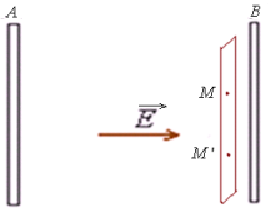
\includegraphics[width=0.3\textwidth]{./img/img_01.png}
\end{wrapfigure}


\subsubsection{Définition}
Le plan équipotentiel est un plan dont tous les point sont au
même potentiel électrique . Ce plan est situé à la même distance
des plaques M et N .

Si un point C a le même potentiel que le point A , on a d’après la
relation précédente : $V_A - V_C = \vec{E}.\overrightarrow{AC} = 0$
donc $V_A \neq 0$ et $V_B \neq 0$, $\vec{E} \perp \overrightarrow{AC}$ 

les plan équipotentiels sont des plans parallèles entre eux et
perpendiculaire au vecteur champ électrique $\vec{E}$

\subsection{ La relation entre l’intensité du champ électrique et la tension :}
On sait que $V_A - V_B = U_{AB}$ qui représente la tension électrique
entre les deux points A et B et d’après la relation précédente :


$V_A - V_B = U_{AB} =  \vec{E}.\overrightarrow{AB}$ = E.AB

$$E = \frac{U_{AB}}{AB}$$


\begin{tcolorbox}[colback=pink!10!white,
                  colframe=blue!15!gray,
                  title=Application -1- :
                 ]
Un champ électrique uniforme d’intensité $E = 3.10^4$ V/m est crée à
l’intérieur de deux plaques parallèles distantes de $d = 10cm$.

  1- Calculer la tension électrique $U_{PN}$ appliquée aux deux
plaques

  2- Déterminer le travail de la force électrique appliquée à un
électron au cours de son déplacement de la plaque N vers la
plaque P .
\end{tcolorbox}

\section{Énergie potentielle électrostatique : }
\subsection{Définition : }
Par analogie à l’énergie potentielle de pesanteur $E_{pp}$ , On définit
aussi l’énergie potentielle électrostatique comme suit :

L’énergie potentielle électrostatique d’une charge q placée en un
point M dans un champ électrique uniforme $\vec{E}$ est donnée par la
relation :
$$E_{pp} = qE.x + Cte$$
et comme E.x = V donc  :
\begin{center}
  \fbox{ 
  $E_{pp}$ = qV + Cte
  }
\end{center}
C est une constante qui dépend du choix de l’origine des potentiels
électriques .

\begin{tcolorbox}
Remarque :
On peut utiliser cette relation pour calculer l’énergie potentielle
électrostatique :

  Epe = qE(x - xref)

  à condition que l’axe x soit orienter vers les potentiels croissants
\end{tcolorbox}
\subsection{Relation entre énergie potentielle électrostatique et travail de la
force électrique : }
On sait que le travail de la force électrique au cours du
déplacement du point A vers le point B , est donné par
l’expression suivante : 
$W_{A\rightarrow B}(\vec{F}) = q(V_A - V_B) $ (1)

et la variation de l’énergie potentielle électrostatique entre A et
B : $\Delta{E_{pp}}  = q(V_B - V_A)$

De ces deux relations , en déduire que :$\Delta{E_{pp}}  = -W_{A\rightarrow B}(\vec{F}) $
 
Cette relation reste valable même si le champ électrique n’est pas
uniforme .
\begin{tcolorbox}[colback=pink!10!white,
                  colframe=blue!15!gray,
                  title=Application -2- :
                 ]
Un champ électrique uniforme d’intensité $E = 103V/m$ est crée
  dans une région de l’espace repérer par $(O, \vec{i},\vec{j}, \vec{k})$ tel que $\vec{E} = E.\vec{i}$

1-Calculer le travail de la force électrique appliquée à un noyau d’hélium $He^{2+}$ du point A(2, 0, 0) vers le point B(4, 2, 0).
L’unité de la longueur est le centimètre .

  2-Calculer l’énergie potentielle électrique au point B . On prend
A comme origine des potentiels.

\end{tcolorbox}

\section{Conservation de l’énergie totale d’une
particule chargée soumise à une force
électrostatique :  }

On considère une particule de charge q et de masse m , se déplace
dans une région de l’espace où règne un champ électrique
uniforme $\vec{E}$ , du point A vers un point B .
D’après le théorème de la variation de l’énergie cinétique entre A
et B et si on néglige le poids de la particule et les forces de
frottement devant la force électrique $\vec{F}$ :
$$\Delta{E_{c}}  = W_{A\rightarrow B}(\vec{F})  $$
et on sait que $\Delta{E_{pp}}  = -W_{A\rightarrow B}(\vec{F}) $
$$ \Delta{E_{c}}  = -\Delta{E_{pp}} $$ 
$$ \Delta{E_{c}(B)} + \Delta{E_{pp}(B)} =  \Delta{E_{c}(A)} + \Delta{E_{pp}(A)} $$ 

On pose : $E_T = E_{C} + E_{pp}$ avec $E_T$ est l’énergie totale de la
particule . Donc on a $E_T(A) = E_T(B)$ i.e qu’on a conservation de
l’énergie totale , donc : $$E_T = \frac{1}{2}. mv^2 + qV$$

v la vitesse de la particule chargée dans le champ $\vec{E}$ et V le
potentiel électrique

L’énergie totale d’une particule de charge électrique q soumise à la
seule action de la force électrique se conserve.

\begin{tcolorbox}[colback=pink!10!white,
                  colframe=blue!15!gray,
                  title=Application -3- :
                 ]
                 Une tension $UAC = 300V$ est appliquée entre l’anode A et la
cathode C d’un canon à électrons.
Des électrons partent de la cathode C sans vitesse initiale, calculer
leur vitesse quand ils arrivent à l’anode A .
  On donne , masse de l’électro $me = 9, 11.10^{-31}kg$
  \end{tcolorbox}

\section{Électron-volt une autre unité d’énergie : }
D’après l’expression du travail de la force électrique appliquée à
une charge électrique qui se déplace d’un point A vers un point B

$W_{A\rightarrow B}(\vec{F})  = q(V_A - V_B) $

Pour un électro on a q = 1e et $V_A - V_B$ = 1V


$W_{A\rightarrow B}(\vec{F})  = 1,6.10^{-19}= 1ev $

En déduit que $1eV =1,6.10^{-19}= 1ev $

cet unité s’appelle électro-volt (eV)
Quelque multiples de l’électron-Volt :
\\$1keV = 10^3 eV$
\\$1MeV = 10^6 eV$
\\$1GeV = 10^9 eV$
\end{document}

